\documentclass{article}
\usepackage{amsmath}
\usepackage{amssymb}
\usepackage{graphicx}
\usepackage{hyperref}
\usepackage[version=4]{mhchem}


\begin{document}
Given \(\triangle A B C, A B=A C, E\) is the midpoint of \(A B\). Extend \(A B\) to \(D\) such that \(B D=B A\). Prove: \(C D=2 C E\).

Solution:
Method 1:\\
Take \(F\), the midpoint of \(C D\). Connect \(B\).\\
Since points \(B, F\) are the midpoints of \(A D, C D\), respectively, \(B F / / A C\) and \(B F=\frac{1}{2} A C\).\\
\centering
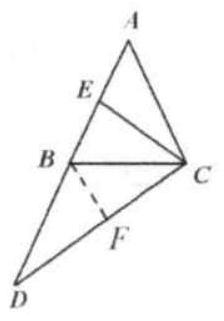
\includegraphics[width=\textwidth]{images/039.jpg}

Since point \(E\) is the midpoint of \(A B, B E=A E\)\\
\(\frac{1}{2} A B==\frac{1}{2} A C=B F\).

Since \(B F / / A C, \angle A=\angle D B F . B D=A B=A C, A E=B F\). \(\triangle A E C \cong \triangle D F B\).\\
\centering
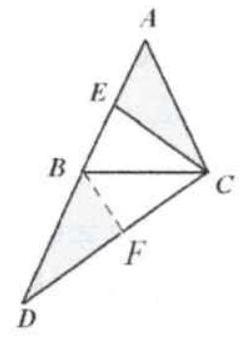
\includegraphics[width=\textwidth]{images/039(1).jpg}

Thus \(D F=C E\), or \(\frac{1}{2} C D=C E \quad \Rightarrow \quad C D=2 C E\).

Method 2:\\
Take \(F\), the midpoint of \(A C\).\\
Connect \(B F\).\\
Since point \(B\) is the midpoint of \(A D, F\) is the midpoint of \(A C\),\\
\centering
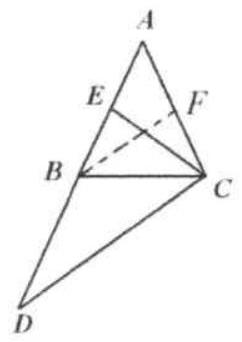
\includegraphics[width=\textwidth]{images/039(2).jpg}

\(B F=\frac{1}{2} D C\)\\
Since \(\triangle A B C\) is an isosceles triangle, \(B F=C E\)\\
Substituting (2) into (1): \(C E=\frac{1}{2} D C \Rightarrow \quad C D=2 C E\).


\end{document}
